\chapter{Implementation}
The solution proposed in Chapters \ref{CHAPTER_proposed_algorithm} and \ref{CHAPTER_combination_with_existings_methods_of_inference} was implemented using the jInfer framework \cite{jinfer}. It is a framework for implementing methods of XML schema inferring created as a software project at Faculty of Mathematics and Physics, Charles University in Prague. It is written in Java as a plugin for NetBeans platform.

The framework consists of modules representing logical parts of a process of inference. The main idea behind the modules is that they can be replaced by other modules with the same interface but different implementation and new modules can be connected to extend functionality.

\begin{figure}
\label{FIG_jinfer}
\caption{jInfer process of inference.}
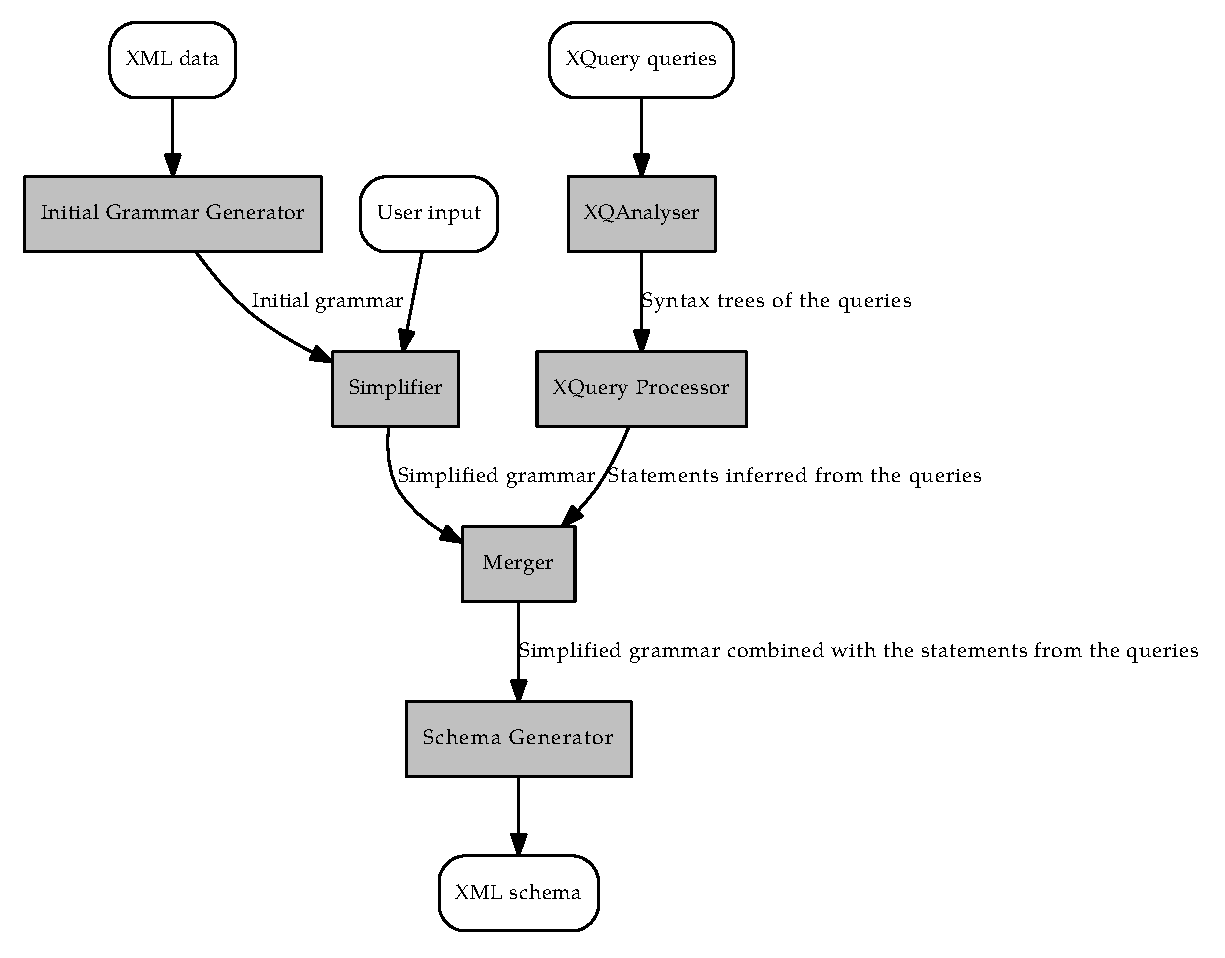
\includegraphics[scale=1]{jinfer.eps}
\end{figure}

Figure \ref{FIG_jinfer} shows the process of inference in jInfer. The grey rectangles represent steps of the inference, the white boxes represent input and output. Originally, the inference was composed of \textbf{Initial Grammar Generator}, \textbf{Simplifier}, and \textbf{Schema Generator} steps. Steps \textbf{XQAnalyzer}, \textbf{XQuery Processor}, and \textbf{Merger} are implementations of main parts of our proposed solution.

\begin{itemize}
\item \textbf{XQAnalyzer} - An implementation of the lexical and syntax analyses proposed in \cite{thesis_schejbal} and modified to create syntax trees. It is partially incorporated in \textbf{XQueryImporter} module (lexer, parser and syntax tree creation) which handles input XQuery files, and \textbf{Base} module (syntax tree data structures) which contains classes shared by several modules.
\item \textbf{XQuery Processor}
\item \textbf{Merger}
\end{itemize}